\documentclass{article}
\usepackage{graphicx}

\begin{flushright}
\begin{tiny}
\textbf{Machine Learning 2: 195 198, 1987}\\
\textbf{© 1987 Kluwer Academic- Publishers, Boston Manufactured in The Netherlands}\\
\end{tiny}
\end{flushright}\\\\\\


\begin{document}
%\maketitle

\begin{flashleft}

\textbf{EDITORIAL}

\end{flashleft}

\textbf{Research Papers in Machine Learning}\\

\begin{small}
\textbf{A prototype for machine learning papers}
\end{small}\\

Scientists do not work in isolation. Communication is central to the
scientific enterprise, and much of the exchange occurs through research
papers. Naturally, the content of these papers will vary with the field of
study, and in this essay I discuss the information that machine learning
researchers should attempt to communicate in their articles. Readers may
interpret these comments as reflecting the current editorial policy of the
journal Machine Learning, though this policy will undoubtedly evolve over
time, as even editors and editorial boards learn from experience.\\

Despite the advantages of standardization, it can lead a new discipline
to crystallize into a rigid pattern before its time. Rather than define an
inflexible format that all papers in machine learning must follow, I provide
below a more flexible, prototypical outline. Specific papers will diverge
from this prototype, but it should provide a useful target, particularly
for authors new to the field. The outline assumes a paper that describes
a single, running machine learning system. Most papers that appear in
Machine Learning will take this form, but later I will briefly consider some
other possibilities.
\\\\\

1. Goals of the research. Machine learning researchers have many different
reasons for carrying out their work. Some are interested in general
principles of intelligent behavior, others are concerned with modeling
human learning, and still others are oriented towards applications. If
an author hopes to communicate with his audience, it is essential that
he state his goals early in the paper, so that readers can decide for
themselves whether the work has made progress towards those goals.\\\\

2. Description of the task. Learning always occurs in the context of some
performance task - such as classification, planning, or language understanding and, for a given performance task, different learning tasks
are possible. For instance, learning from examples and conceptual clustering both involve classification, but they differ in the information
given and in the nature of the learned structures. The author should
clearly state both the performance and learning tasks he is studying,
specifying the given inputs and the desired outputs.
196 P. LANGLEY \\\\\
3. Representation. Any learning system must represent its inputs - the
data and knowledge on which learning is based - and its outputs the
knowledge it acquires. The author should describe the representational
scheme used for both types of information.\\\\\
4. Performance component. Learning involves some improvement in performance, and the author should describe the system's performance
element in enough detail to support description of the learning method.\\\\\
5. Learning algorithms. Naturally, the learning method should be a central focus of any paper on machine learning. The author should clearly
describe the basic steps of the learning mechanism under study, using
flow charts or English paraphrases of the algorithm to supplement the
text. Ideally, he should describe the learning method in sufficient detail to let readers reconstruct the system on their own. The ability to
replicate results is essential to any true science.\\\\\
6. Detailed examples. No matter how clear the abstract description of a
learning algorithm, it can always be clarified by examples. The author
should include at least one detailed example of his method in operation.
Figures accompanied by text usually communicate such examples far
better than do program traces.\\\\\
7. Evaluation. Without some evaluation of the learning method, readers
cannot know whether the work constitutes a step forwards or backwards. This section is central to any machine learning paper. Of
course, one can imagine a variety of evaluation schemes, differing according to the author's goals. The most obvious alternatives are:
o Empirical evaluation. This approach tests the learning algorithm's
behavior empirically under varying conditions and using different
metrics. For instance, one might show that the time taken to
converge on useful structures degrades with increases in noise.
o Theoretical evaluation. This approach proves theorems about the
behavior of learning algorithms. For example, one might show that
the number of instances needed to acquire the correct structure
increases as a polynomial function of the structure's complexity.
o Psychological evaluation. This approach compares the algorithm's
behavior to human learning behavior. For example, a given model
might explain the power law of practice, a phenomenon that has
been observed in human skill acquisition across many domains.
Note that these methods are not contradictory; one can evaluate a
single method along all three dimensions. One can also imagine other
evaluation schemes, and the field has plenty of room for alternative
paradigms; however, all such paradigms should be based on some principled evaluation techniques. The issue of generality cuts across all
such paradigms, and authors should attempt to characterize the class
of tasks for which their results hold.\\\\\\\\

\begin{small}
\textbf{RESEARCH PAPERS IN MACHINE LEARNING 197}
\end{small}\\

\begin{figure}
    \centering
   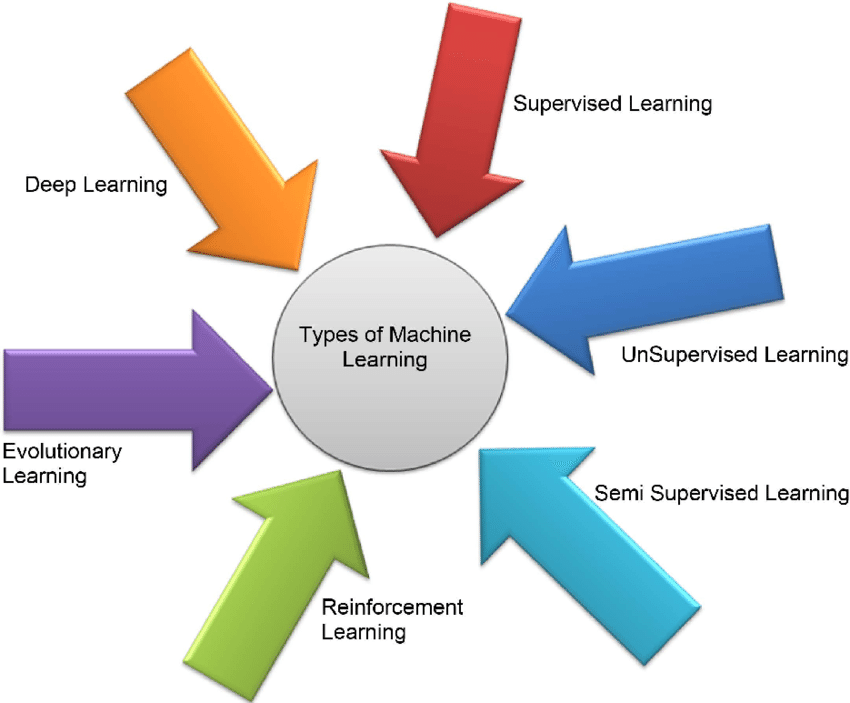
\includegraphics[width=0.8\linewidth]{Types-of-machine-learning-techniques.png}
       \caption{Types of machine learning technic}
    \label{fig:Diffrent type of machine learning}
\end{figure}
8. Related work. Ideas never occur in a vacuum, and the methods described in a paper will invariably bear an interesting relation to earlier
research. The author should describe how his approach differs from
its predecessors and how it is similar. He should also point out the
contribution of both the earlier and the current work.\\\\\
9. Future research. Science is a never-ending process, and no matter how
impressive a given piece of research, there is always more work to be
done. The author should clearly state the limits of his approach to
learning and list the questions he has failed to answer. He should then
outline his plans for remedying these drawbacks in future efforts.
The order of these sections is less important than their content, though
clearly some should precede others. The author need not divide the material in precisely this fashion, provided he presents the information in
some manner. But the above outline should serve as a useful prototype for
research papers on machine learning.\\\\\

\begin{small}
\textbf{Machine learning as an empirical science}
\end{small}\\

One of the evaluation techniques mentioned above involved the empirical
study of an algorithm's behavior, and this approach is prevalent enough
within machine learning to deserve further discussion. Most sciences are
empirical in nature, and this means their theories are based on robust empirical phenomena, such as the law of combining volumes and the ideal gas
law. A growing number of machine learning researchers are focusing their
efforts on discovering analogous phenomena in the behavior of learning
systems, and this is an encouraging sign.
In many sciences, such phenomena are stated in terms of relations between independent and dependent variables.1
 In machine learning, two natural independent terms are the structure of the knowledge to be learned and
the regularity in the environment (e.g., the amount of noise in the data).
For incremental learning methods, one may also vary the order in which
data are presented and the stability of the environment over time. Most
natural dependent measures are related to some performance criterion,
such as diagnostic accuracy (for classification tasks) or quality of solution
paths (for problem-solving tasks). However, these are not the only such
variables, and one important task awaiting machine learning researchers is
the identification of relevant independent terms and useful metrics.
Recent work along these lines has been carried out by Quinlan (1986),
Fisher (1987), and others. Although much of the experimental work has
examined the behavior of empirical learning methods, it can also be applied to explanation-based techniques, and O'Rorke (1987) reports a set
1Of course, simply collecting data is not enough; empirical results are useful only to
the extent that they lead to deeper understanding.
198 P. LANGLEY
of experiments within this framework. In other words, the experimental
evaluation of learning algorithms is a general approach that can be usefully
applied to all machine learning paradigms.\\\\\\\\\

\begin{small}
\textbf{Other types of machine learning papers}
\end{small}\\\\

\begin{figure}
    \centering
   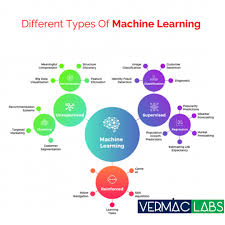
\includegraphics[width=0.8\linewidth]{types of Machine learning.jpg}
       \caption{Diffrent type of machine learning}
    \label{fig:Diffrent type of machine learning}
\end{figure}

apers that diverge from the prototype outlined above may still contribute to the field. For instance, articles that compare the empirical behavior of different algorithms (e.g., Schlimmer & Fisher, 1986) will necessarily spend less time describing the methods themselves and more time
discussing their behavior. Purely theoretical papers (e.g., Rivest, 1987)
may focus on task characteristics that hold for all algorithms, and thus\\\\\
\section{Classic AI Technic for Deep Rainforcement}

\begin{tabular}{|c|c|c|}

\hline
\textbf{Classification} & \textbf{Regression} & \textbf{Clustering} \\
\hline
Support Vector Machines & Linear Regression & K-Means \\
\hline
Discriminant Analysis & SVR & Fussy C-Means \\
\hline
Naive Bayes & Decision Trees & Hidden Markov Model \\
\hline
Nearest Neighbour & Neural Networks & Hebbian Learning \\
\hline
\end{tabular}\\\\
devote their discussion to statements and proofs of theorems.
Syntheses of earlier results also have a role to play, since they can reveal
underlying connections between tasks and methods that were previously
thought disparate. Such papers need not present any new empirical results, but they will prove more useful to the extent that they suggest new

variations on tasks and methods. Naturally, the threshold for accepting
survey papers should be higher than that for alternative formats.
Machine learning is an evolving discipline, and the nature of its research
papers must change along with the interests of its constituents. But hopefully, the formats and evaluation criteria outlined above will serve the field
well for some years to come, as we explore the empirical, theoretical, and
psychological facets of learning.

\\\\\\\\\

\begin{flushright}
\textbf{Pat Langley}\\
\textbf{University of California, Irvine}\\
\textbf{Langley@CIP.UCI.EDU}\\
\end{flushright}

\begin{flushleft}
\textbf{References}\\
\end{flushleft}

\begin{tiny}
Fisher, D. H. (1987). Knowledge acquisition via incremental conceptual clustering.\\
Machine Learning, 2, 139-172.\\
O'Rorke, P. (1987). LT revisited: Experimental results of applying explanation\\based learning to the logic of Principia Mathematica. In Proceedings of the\\
Fourth International Workshop on Machine Learning (pp. 148-159). Irvine,\\
CA: Morgan Kaufmann.
Quinlan, J. R. (1986). Induction of decision trees. Machine Learning, 1, 81-106.\\
Rivest, R. L. (1987). Learning decision lists. Machine Learning, 2, 229-246.\\
Schlimmer, J. C., & Fisher, D. H. (1986). A case study of incremental concept\\
induction. Proceedings of the Fifth National Conference on Artificial Intelli\\gence (pp. 496-501). Philadelphia, PA: Morgan Kaufmann.\\
\end{tiny}


\end{document}